%
% $Id$
%
% Design for loaddods

\documentclass{article}
\usepackage{epsfig}
\usepackage{rotating}
\usepackage{subfigure}
\usepackage{vcode}
\usepackage{xspace}

% Change paragraph typesetting; eliminate indenting and add more space between
% paragraphs. 2/15/2000 jhrg
\setlength{\parindent}{0em}     % Amount of indentation
\addtolength{\parskip}{1ex}     % Vertical separation

\newcommand{\Cpp}{\rm {\small C}\raise.5ex\hbox{\footnotesize ++}\xspace}
\newcommand{\dap}{\rm {\small DAP}\raise.5ex\hbox{\footnotesize ++}\xspace}
\newcommand{\maewesturl}{http://maewest.gso.uri.edu/\-cgi-bin/\-nph-dsp/\-htn\_sst\_decloud/\-1992/\-i92098065016.htn\_d.Z\xspace}

\begin{document}

\title{Matlab Loaddods Requirements and Design}
\author{James Gallagher\thanks{The University of Rhode Island,
    jgallagher@gso.uri.edu}}
\date{\today \\ $Revision$ }

\maketitle
\tableofcontents

\section{Introduction}

This paper is a combination requirements and design document for the Matlab
version of \texttt{loaddods}. Initially, I wrote loaddods quickly and without
any formal requirements or design in Nov. 1997. The program has been expanded
many times since then. It seemed like a design of some sort would simplify
adding new features and that, combined with the need to add support for the
DAS and DDS objects, lead to this paper.

Because of the backwards nature of the development of loaddods, in this paper
I include only the new requirements for loaddods and the design that
implements them. the base version of loaddods cooresponds to version 3.1. To
provide a framework in which to preset the requirements and design, I include
a section on the current (that is, version 3.1) architecture of loaddods
first, before the requirements or design. This seems to make the most sense
since the software already exists; pretending that all the requirements were
written before the software seems silly.
% Because of the backwards nature of the development of loaddods, in this paper
% I include only the requirements for loaddods and the design that implements
% them. To provide a framework in which to preset the requirements and design,
% I include a section on the current architecture of loaddods first, before the
% requirements or design. This seems to make the most sense since the software
% already exists; pretending that the requirements were written before the
% software seems silly.

Section~\ref{sec:arch} describes the architecture of loaddods, including how
loaddods and writeval work together.

Section~\ref{sec:requirements} describes the new requirements.

Section~\ref{sec:design} describes how those requirements are satisfied.

\section{Architecture of the Matlab loaddods command}
\label{sec:arch}

The Matlab (ML) loaddods client is made of two programs that communicate
asynchronously using a UNIX pipe. The writeval program is a true DODS client
program built using the \dap \Cpp class library. This DODS client
dereferences one or more DODS URLs and writes the returned data to standard
output using the grammar shown in Table~\ref{tab:writeval-grammar}.
The second program is the ML Mex program \texttt{loaddods}. This program reads the
output from writeval and interns each variable into the ML caller
workspace.

The loaddods client is split into two programs because of difficulties
building ML Mex programs written in \Cpp\footnote{Actually, the design was
  first a quick work-around for a DNS problem at MIT, but it became important
  for the other reasons mentioned here.}. Originally loaddods ran under ML
4\footnote{We no longer support ML 4.} and it was not possible to write Mex
programs in \Cpp. Matlab 5 does support \Cpp Mex programs, but only if
certain \Cpp compilers are used and, for each UNIX platform, a different
compiler is required. Since we use Gnu gcc for all our platforms, satisfying
this requirement of ML would mean a major shift in the way we develop DODS.
For this reason loaddods will stay implemented as two separate programs for
the foreseeable future.

Figures~\ref{fig:loaddods-component}~and~\ref{fig:loaddods-writeval-activity}
show how these two programs interact. The writeval program is started by
loaddods in a child process and a pipe connects the output of writeval to the
input of loaddods. It is passed a URL and various command options based on
the options\footnote{See Appendix~\ref{app:options} for a description of
  loaddods' options.} sent to loaddods by the user. writeval then
dereferences the URL and begins writing to the pipe.  loaddods reads the
values and decides how to intern them based on the options with which it was
called.

\begin{figure}
\begin{center}
\epsfig{file=loaddods-deployment.eps,width=5in}
\caption{UML Deployment Diagram showing the software components involved with
  DODS access using Matlab. loaddods and writeval communicate over a UNIX
  pipe using a grammar described in Table~\ref{tab:writeval-grammar}.
  writeval makes requests of DODS servers and returns values to loaddods
  via the pipe.}
\label{fig:loaddods-component}
\end{center}
\end{figure}

\begin{figure}
\begin{center}
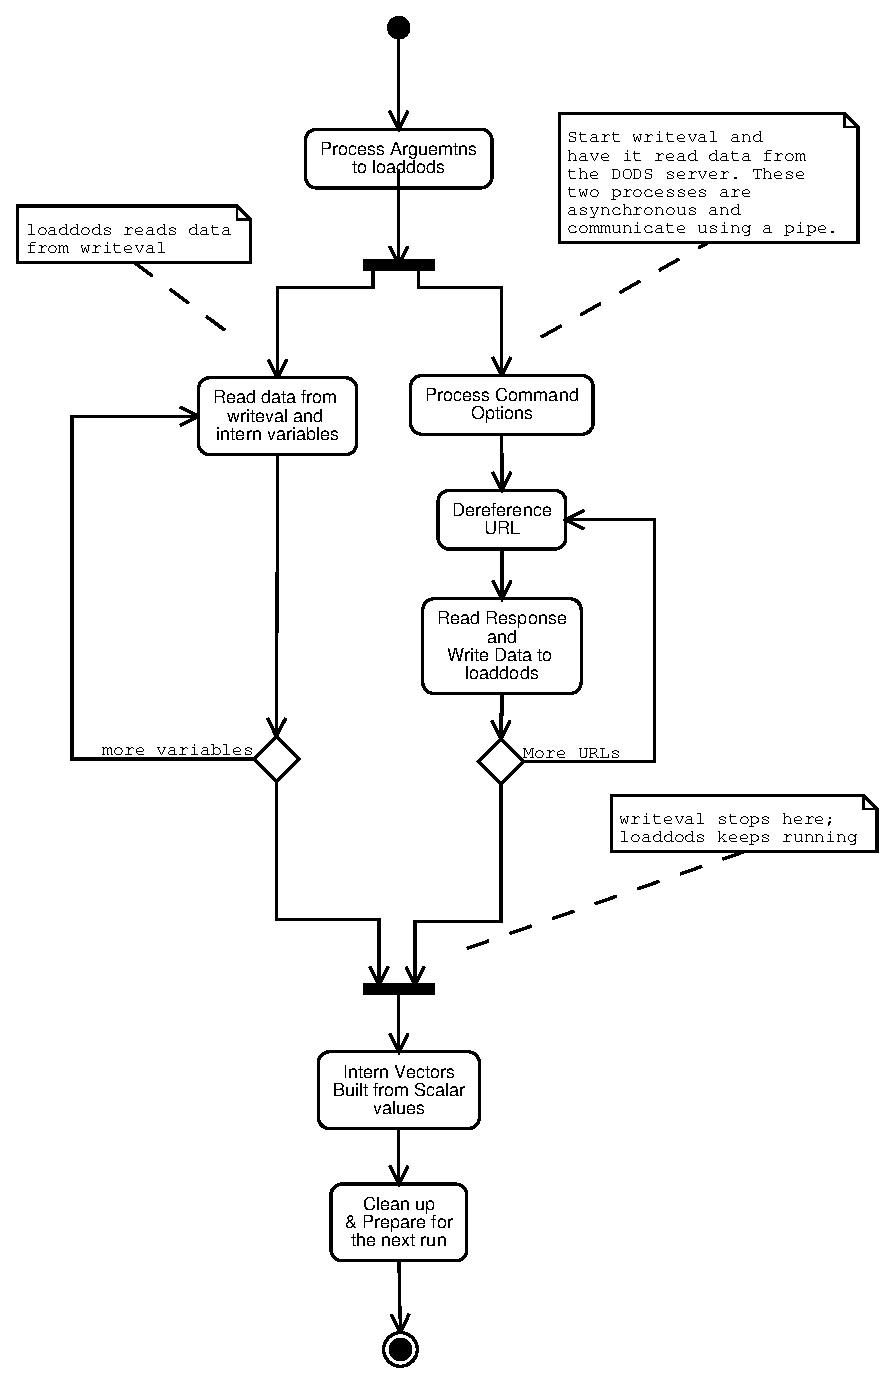
\epsfig{file=loaddods-writeval-activity.eps,height=7in}
\caption{UML Activity diagram for the loaddods Mex command and writeval DODS
  client. These two programs comprise the `Matlab loaddods client'.}
\label{fig:loaddods-writeval-activity}
\end{center}
\end{figure}

\begin{table}

\caption{Grammar for the output of writeval. It uses this grammar to write
  values to a UNIX pipe from which loaddods reads. The information written
  contains a mixture of ASCII and binary data (but see writeval's -a option
  for a pure ASCII version of this output). The grammar was designed to be
  easy to parse while still maintaining all of the hierarchy information
  present in the DDS object.}
\label{tab:writeval-grammar}
\begin{minipage}{\linewidth}
\begin{center}
\begin{tabular} {|rcl|} \hline
\emph{data-request} 
& $\rightarrow$ & \emph{variable*} \\ \hline

\emph{variable} 
& $\rightarrow$ & \emph{simple-variable} \\
& $\rightarrow$ & \emph{vector-variable} \\
& $\rightarrow$ & \emph{constructor-variable} \\ \hline

\emph{simple-variable} 
& $\rightarrow$ & \texttt{Byte} \emph{nl}\protect\footnote{The newline character.} \emph{variable-name} \emph{nl} \emph{data} \emph{nl} \\
& $\rightarrow$ & \texttt{Int32} \emph{nl} \emph{variable-name} \emph{nl} \emph{data} \emph{nl} \\
& $\rightarrow$ & \texttt{Float64} \emph{nl} \emph{variable-name} \emph{nl}  \emph{data} \emph{nl} \\
& $\rightarrow$ & \texttt{String} \emph{nl} \emph{variable-name} \emph{nl} \emph{string-data} \emph{nl}\\ 
& $\rightarrow$ & \texttt{Url} \emph{nl} \emph{variable-name} \emph{nl} \emph{string-data} \emph{nl} \\ \hline

\emph{vector-variable} 
& $\rightarrow$ & \texttt{Array} \emph{nl} \emph{array-variable} \emph{nl} \emph{data} \\
& $\rightarrow$ & \texttt{List} \emph{nl} \emph{list-variable} \emph{nl} \emph{data} \\ \hline

\emph{constructor-variable} 
& $\rightarrow$ & \texttt{Structure} \emph{nl} \emph{struct-variable} \\
& $\rightarrow$ & \texttt{Sequence} \emph{nl} \emph{sequence-variable} \\ 
& $\rightarrow$ & \texttt{Grid} \emph{nl} \emph{grid-variable} \\ \hline

\emph{string-data} 
& $\rightarrow$ & \emph{string} \emph{nl} \\ \hline

\emph{array-variable} 
& $\rightarrow$ & \emph{variable-type} \emph{variable-name}
\emph{number-of-dims} \emph{nl} \emph{dim-size}+\protect\footnote{The number of
  dimension sizes must match the value of \emph{number-of-dims}.} \\ \hline

\emph{list-variable} 
& $\rightarrow$ & \emph{variable-type} \emph{variable-name} \emph{list-size} \\ \hline

\emph{struct-variable} 
& $\rightarrow$ & \emph{variable-name} \emph{num-of-elements} \emph{nl} (\emph{variable})+ \\ \hline

\emph{sequence-variable} 
& $\rightarrow$ & \emph{variable-name} \emph{num-of-columns} \emph{nl} (\emph{variable})+ \\ \hline

\emph{grid-variable}
& $\rightarrow$ & \emph{variable-name} \emph{nl} \texttt{array} \emph{nl} \emph{array-variable} \\
& & \texttt{map} \emph{num-of-arrays}\emph{nl} (\emph{array-variable})+  \\ \hline

\emph{error} 
& $\rightarrow$ & \texttt{Error} \emph{nl} \emph{message} \emph{nl} \\ \hline

\emph{attribute} 
& $\rightarrow$ & \texttt{Attribute} \emph{nl} \emph{dataset-name} \emph{nl}
\emph{num-of-containers} \\ 
& & \emph{nl} (\emph{struct-variable})+ \\ \hline

\end{tabular}
\end{center}
\end{minipage}
\end{table}

\section{Requirements}
\label{sec:requirements}

Two new groups of requirements are being added to loaddods. The first changes
the way attribute information is accessed by the program. This replaces
previous behavior that was conceptually flawed. The new feature reads
attribute information and presents it to the user as a Matlab 5 structure
variable. The hierarchy of the DDS object is superimposed on the DAS so that
all of the information in both objects is available in one ML variable.

Unlike loaddods' treatment of variables, the only supported way to intern the
attribute information is by assigning the return value of loaddods to a ML
variable. This is in contrast to the way variable are interned in ML; most
values are stored in variables created and added to the ML workspace by
loaddods. It is possible to assign values read using loaddods to variable
(and thus choose the variables' names), but since it has previously been
hard to know what exactly would be returned in response to a query, this
option was rarely used.

The second new feature for loaddods is an option which will return all
requested variables as fields in a single ML structure variable. Thus,
regardless of the number of variables returned by a request, it will always
be possible to assign the return values to a single ML variable. In addition,
this option will preserve the hierarchy of the variables, information which
is currently discarded.

The command options which access these new features are shown in
Table~\ref{tab:loaddods-options}. The table also shows which features are
currently implemented. Specific requirements for the -A option are given in
section~\ref{sec:attributes} and requirements for -Q are given in
Section~\ref{sec:variables}. 

\begin{table}
\caption{The new loaddods switches and their behavior.}
\label{tab:loaddods-options}
\begin{center}
\begin{tabular}{|ll|c|} \hline
\sc{Syntax} & \sc{Operation} & \sc{Implemented} \\ \hline
X = loaddods(URL?constraint);
& Writes data structure called X & \sc{No}\\
& using DataDDS to name fields. & \\

loaddods(URL?constraint);
&  Spews out unstructured variables & \sc{Yes}\\
&  directly into the workspace. & \\

\hline

X = loaddods('-Q', URL?constraint);
& Writes data structure called X & \sc{No}\\
& using DataDDS to name fields. &\\

X = loaddods('-Q',URL);
& Downloads whole dataset into a & \sc{No}\\
& structure named X.&\\ 

loaddods('-Q',URL[?constraint])
& Returns an error & \sc{No}\\

\hline

X = loaddods('-A',URL);
& Writes combined DAS/DDS into & \sc{Yes}\\
& a structure named X. &\\

X = loaddods('-A',URL?constraint);
& Ignores constraint and reads entire & \sc{Yes}\\
& DAS/DDS into a structure named X. & \\

loaddods('-A',URL[?constraint])
&  returns an error & \sc{Yes}\\

\hline

\end{tabular}
\end{center}
\end{table}

\subsection{Accessing dataset attributes}
\label{sec:attributes}

The Matlab loaddods client cannot currently read either the DDS or DAS
information in a way that makes that information easy to use. This
information is important because we plan to use metadata for the DAS and DDS
to eliminate a development and scalability bottleneck in the current ML GUI
client and to facilitate the development of other sophisticated clients.

The metadata in the DAS and DDS objects will be used two ways: to understand
what is available from a dataset before reading actual data values and to
transform data values read into a normalized data space (e.g., to change
from byte counts to degrees C). 

Section~\ref{sec:complete-dataset} describes reading and interning
attributes for a complete dataset. 

See Appendix~\ref{app:dds-das} for a sample DDS and DAS from a real dataset
as well as the way that information will be interned in ML.

\subsubsection{Attributes for a complete dataset}
\label{sec:complete-dataset}
\begin{enumerate}
\item To access DAS/DDS information for an entire dataset, use the -A option
  with loaddods.\footnote{This option is used for the currently broken
    attribute support. That support will be fixed/changed to the scheme
    described here.} See Appendix~\ref{app:dds-das} for samples of
  the interned data structure.
\item Attribute and datatype information for each variable in the dataset will
   be stored in a ML structure variable whose name is the same as the
   dataset's.
\item Do not create fields for synthesized variables (e.g., Grid maps which
  are duplicated outside  the Grid).
\item For each variable in the DDS:
\begin{enumerate}
\item Create a matching structure element.
\item Within this structure, create a vector field named
  \texttt{DODS\_ML\_Size} which will hold the dataset dimension information
  of this variable.
\item Because variable names in DODS may contain characters which are illegal
  in ML, writeval translates the illegal characters into underscores.
  However, loaddods must be able to form URLs which ask for variables by name
  and since any illegal character is mapped to an underscore, it cannot do
  that using the variable names as the are presented in the ML workspace. To
  support building URLs, each variable has a \texttt{DODS\_ML\_Real\_Name}
  field that contains the exact character sequence of the variable's name on
  the DODS server. Note that this string may contain percent (\%) characters
  since that is how HTTP escapes unprintable characters in URLs.
\item Also, for each variable add a field for each attribute:
\begin{enumerate}
\item The name of the field will be the name of the attribute.
\item The value of the field will be the value of the attribute.
\item A String attribute will map to ML strings.
\item A numeric attribute will map to ML floats.
\item A vector attribute will map to a vector of the corresponding ML type.
\item A container attribute will map to a ML Structure.
\end{enumerate}
\end{enumerate}

\item To encode the dataset's global attributes:\footnote{Global attribute are
    defined as those attributes that correspond to no variable in the
    dataset.}
\begin{enumerate}
\item Make a structure called \texttt{global} to hold all the dataset's
  global attribute containers.
\item Intern global attributes as fields within the \texttt{global}
  structure.
\item The structure of the global attributes in the DAS will be replicated in
  the \texttt{global} structure.
\end{enumerate}

\end{enumerate}

\subsubsection{Using \texttt{loaddods} to get attribute information}

To access the DAS information using loaddods, a new option will be added to
the client program. In addition, a new option for accessing data will also be
added. Table~\ref{tab:loaddods-options} lists these along with their
behavior.

\subsection{Variable access that preserves hierarchy }
\label{sec:variables}

This section will be written once time is allocated to start the work.

\section{Design and Implementation}
\label{sec:design}

TODO: Describe each class.

\begin{figure}
\begin{center}
\epsfig{file=loaddods-activity-new.eps,height=8.0in}
%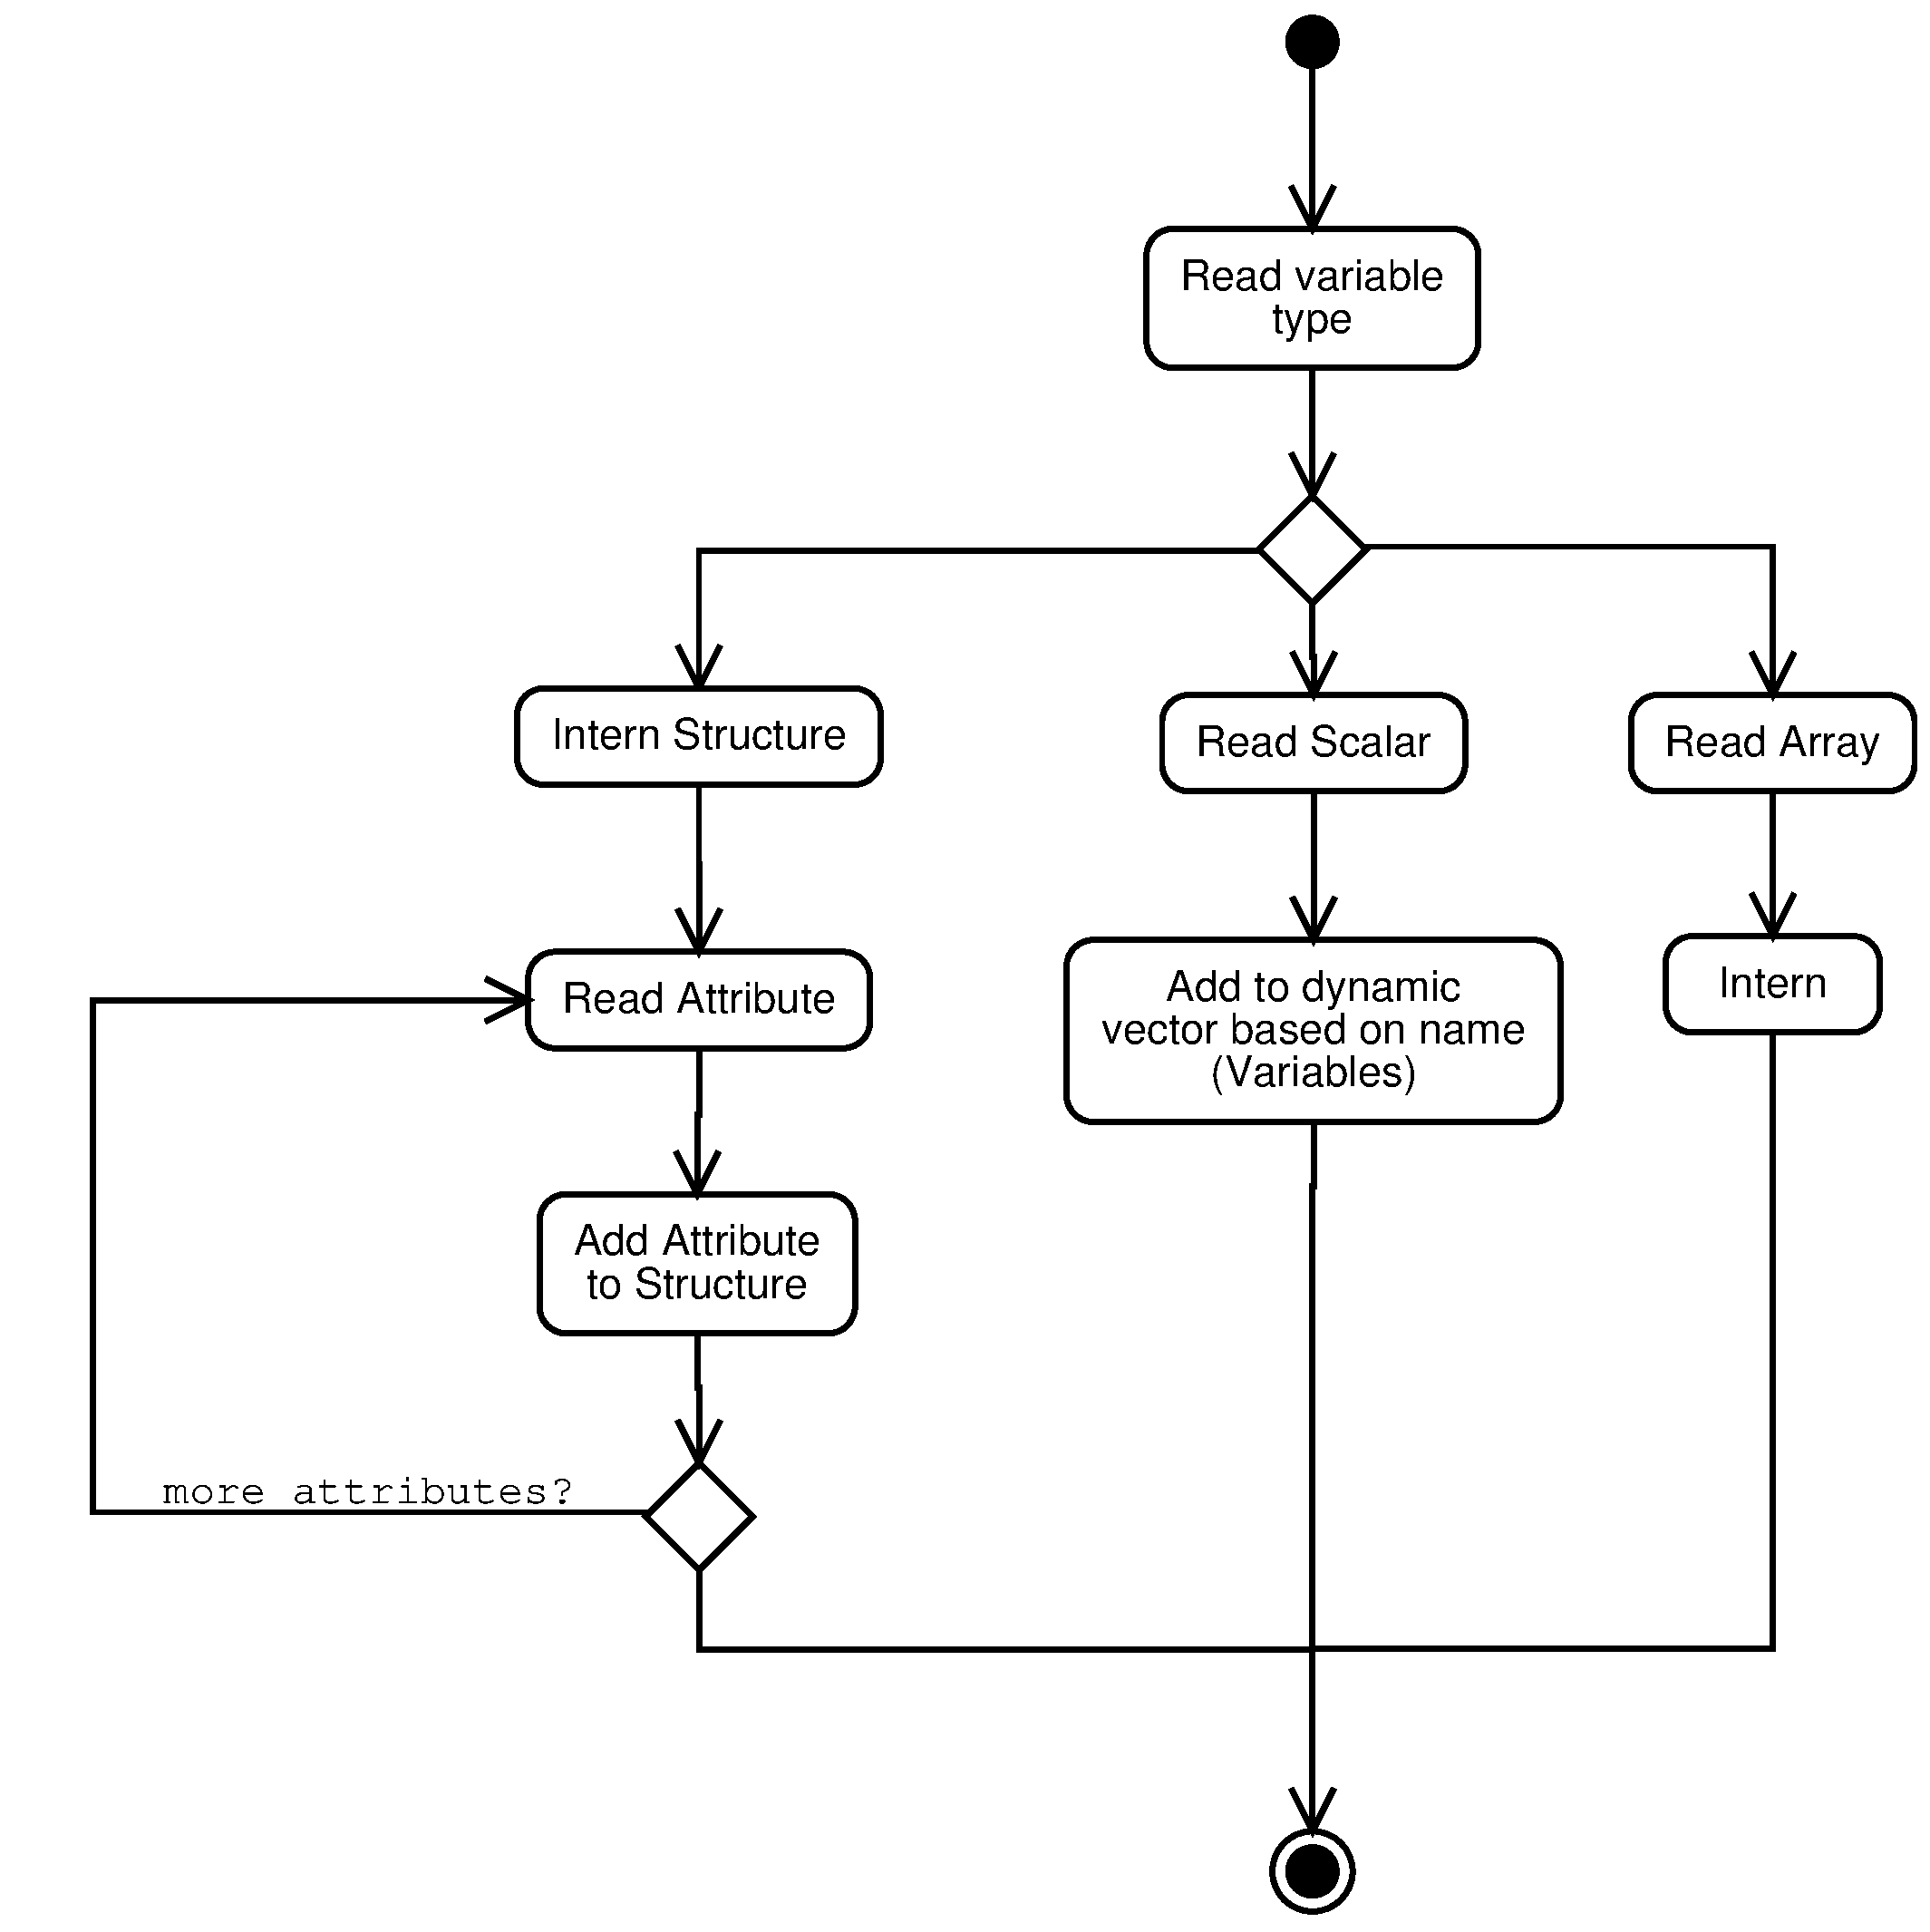
\epsfig{file=intern-with-attr.eps,width=3in}
\caption{Addition to the loaddods data stream processing loop to incorporate
  handling attribute information.}
\label{fig:loaddods-attr-processing}
\end{center}
\end{figure}

Figure~\ref{fig:loaddods-class} shows a pseudo class diagram for
loaddods.\footnote{Pseudo since loaddods is actually a C program; but the
  source files are class-like.} 

\begin{sidewaysfigure}
\begin{center}
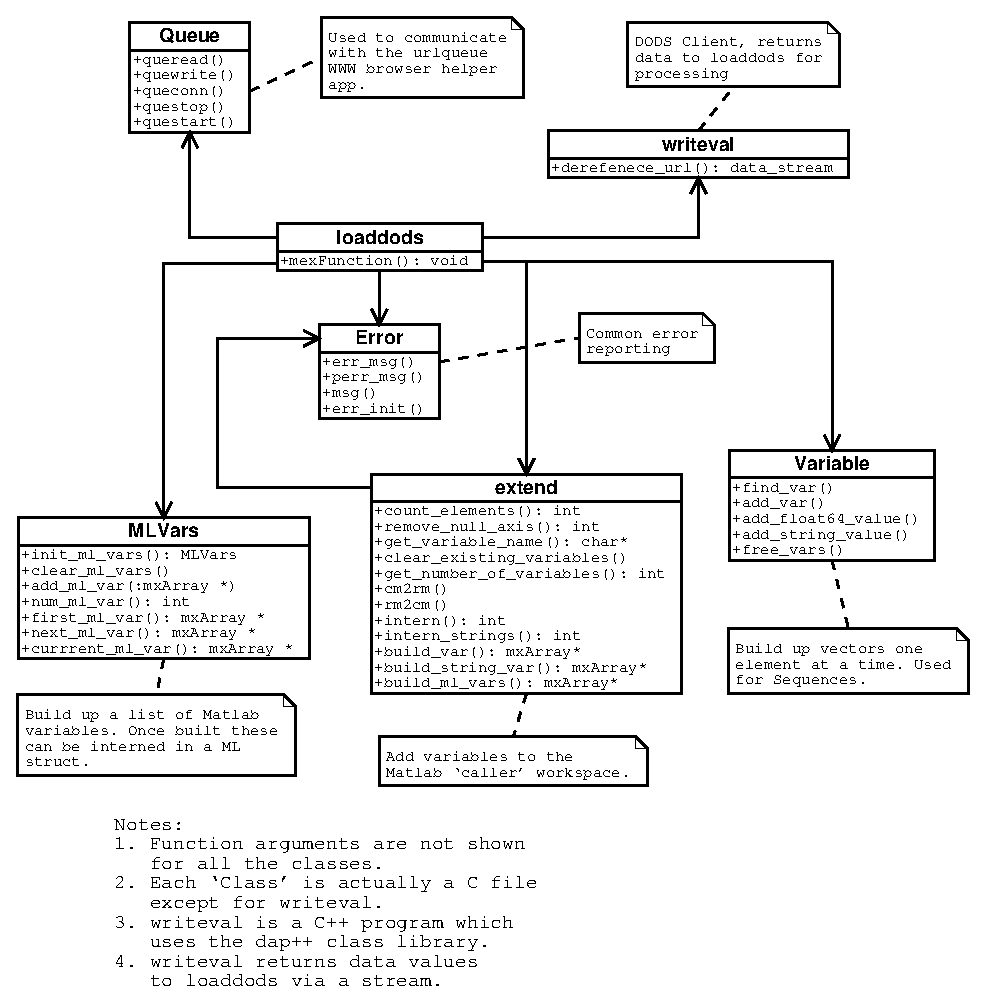
\epsfig{file=loaddods-files.eps,height=5.0in}
\caption{UML class diagram for loaddods. The writeval program is shown as a
  class.}
\label{fig:loaddods-class}
\end{center}
\end{sidewaysfigure}

Figure~\ref{fig:writeval-datatypes} shows how the attribute information will
be combined with the DDS. \Cpp's multiple inheritance will be used to add an
instance of the class \texttt{AttrTable} to each of the derived classes
\texttt{ClientByte}, \ldots, \texttt{ClientGrid}. 

\begin{sidewaysfigure}
\begin{center}
\epsfig{file=writeval-datatype-proposed-class.eps,height=5.0in}
\caption{UML Diagram for the structure of \texttt{writeval}'s datatype
  organization. The classes \texttt{ClientByte}, etc., will inherit from both
  \texttt{Byte}, etc., and \texttt{AttrTable}. Other software will transfer
  attribute information from the DODS server's DAS object to the new
  `amplified' variables.}
\label{fig:writeval-datatypes}
\end{center}
\end{sidewaysfigure}

Figure~\ref{fig:writeval-org} shows the organization of writeval. Even though
writeval itself is not a class, I've shown it as such. The class
\texttt{MetadataProcessing} is used to move the attribute information from
the DAS to the new variables.

\begin{sidewaysfigure}
\begin{center}
\epsfig{file=writeval_implementation.eps,width=8.0in}
\caption{UML Diagram for \texttt{writeval}. The class
  \texttt{MetadataProcessing} handles moving DAS information into variables.}
\label{fig:writeval-org}
\end{center}
\end{sidewaysfigure}

\clearpage
\appendix

\section{Example DAS and DDS objects}
\label{app:dds-das}

The DDS and DAS objects for the dataset \texttt{\maewesturl} are shown in
Figure~\ref{fig:dds-das}. Note that the DAS containers do not reflect the
nesting of variables in the DDS and that the DDS has duplicates of the Grid
map vectors \texttt{lat} and \texttt{lon} at the dataset's top level.

\begin{figure}[!]
\begin{scriptsize}
\subfigure[DAS]{\begin{vcode}{i}
Attributes {
    lat {
        String units "degrees_north";
        String long_name "latitude";
    }
    lon {
        String units "degrees_east";
        String long_name "longitude";
    }
    dsp_band_1 {
        Byte dsp_PixelType 1;
        Byte dsp_PixelSize 1;
        Int32 dsp_Flag 0;
        Int32 dsp_nBits 8;
        Int32 dsp_LineSize 0;
        String dsp_cal_name "Temperature";
        String units "Temp";
        Int32 dsp_cal_eqnNumber 2;
        Int32 dsp_cal_CoeffsLength 8;
        Float64 dsp_cal_coeffs 0.125, -2.;
        Float64 scale_factor 0.125;
        Float64 add_off -2.;
    }
    NC_GLOBAL {
        Int32 dsp_SubImageId 0;
        Int32 dsp_ModificationDate 19990104;
        .
        .
        .
    }
}
\end{vcode}
}
\subfigure[DDS]{\begin{vcode}{i}
Dataset {
    Grid {
     ARRAY:
        Byte dsp_band_1[lat = 1024][lon = 1024];
     MAPS:
        Float64 lat[lat = 1024];
        Float64 lon[lon = 1024];
    } dsp_band_1;
    Float64 lat[lat = 1024];
    Float64 lon[lon = 1024];
} i92098065016;
\end{vcode}
}
\end{scriptsize}
\caption{The DDS and DAS for \texttt{\maewesturl}.
    Most of the attributes in the NC\_GLOBAL container have been elided.}
\label{fig:dds-das}
\end{figure}

The Figure~\ref{fig:ideal-organization} shows how the DDS and DAS in
Figure~\ref{fig:dds-das} should look once interned in Matlab. Note that the
dataset using in this example has one global attribute container called
\texttt{NC\_GLOBAL} and that is a structure within the structure
\texttt{global}. If the dataset had several global attribute containers
(maybe one from the dataset and one added using an ancillary attribute
object) those additional containers would be fields in \texttt{global}.

\begin{figure}
\begin{scriptsize}
\subfigure[]{\begin{vcode}{i}
i92098065016 = 

        global: [1x1 struct]
    dsp_band_1: [1x1 struct]

i92098065016.global.NC_GLOBAL =

          dsp_SubImageId: 0
    dsp_ModificationDate: 19990104
    dsp_ModificationTime: 200639
        dsp_SubImageFlag: 64
       dsp_SubImageTitle: 'Ingested by SCRIPP'
           dsp_StartDate: 19920407
           dsp_StartTime: 6.5017e+04
               dsp_SizeX: 1024
               dsp_SizeY: 1024

i92098065016.dsp_band_1 =

  DODS_ML_Real_Name: 'dsp_band_1'
         dsp_band_1: [1x1 struct]
                lon: [1x1 struct]
                lat: [1x1 struct]
\end{vcode}
}
\subfigure[]{\begin{vcode}{i}
i92098065016.dsp_band_1.dsp_band_1 =

           dsp_PixelType: 1
           dsp_PixelSize: 1
                dsp_Flag: 0
               dsp_nBits: 8
            dsp_LineSize: 0
            dsp_cal_name: 'Temperature'
                   units: 'Temp'
       dsp_cal_eqnNumber: 2
    dsp_cal_CoeffsLength: 8
          dsp_cal_coeffs: [0.1250 -2]
            scale_factor: 0.1250
                 add_off: 2
            DODS_ML_Size: [1024 1024]
       DODS_ML_Real_Name: 'dsp_band_1'

i92098065016.dsp_band_1.lon =

              units: 'degrees_east'
          long_name: 'longitude'
       DODS_ML_Size: 1024
  DODS_ML_Real_Name: 'dsp_band_1'

i92098065016.dsp_band_1.lat =

              units: 'degrees_north'
          long_name: 'latitude'
       DODS_ML_Size: 1024
  DODS_ML_Real_Name: 'dsp_band_1'
\end{vcode}}
\end{scriptsize}
\caption{Ideal organization of DAS and DDS information, taken from Matlab
    using a mockup of information from the source used in Figure~\ref{fig:dds-das}.}
\label{fig:ideal-organization}
\end{figure}

\section{Options for loaddods---Implemented and planned}
\label{app:options}

\subsection{loaddods}
The \texttt{loaddods} Matlab command has several forms:
\begin{description}
\item[loaddods(\emph{switches}, URL \emph{url options}, \emph{URL url options});]
  This is the main form of a loaddods command. The URL parameter is required,
  the switches are optional as are second, third, \ldots URLs.
  
\item[arg = loaddods('-A', URL);] When using the -A (Attributes) option you
  \emph{must} supply a return argument.

\item[a1 a2 \ldots an = loaddods(\ldots);] Loaddods can be used to access
  variables and assign them to a vector of arrays. Also, note that the -s
  option can be used to load the first of the return value with the DODS
  names of each subsequent return argument. If $m$ return values are
  requested via the URL's constraint, but only $n$ (where $m>n$) argument are
  given, the excess return value are silently discarded.\footnote{The -Q
    option will probably make this form of the command obsolete.}

\item[loaddods;] Run loaddods but wait for a URL to be sent via a UNIX queue.
  This form of the command is meant to work with web browsers and other
  programs. In the case of a web browser, an interface would return a URL to
  the browser wrapped in a MIME document which is routed to a helper
  application which in turn sends the URL to the queue. This is hardly ever
  used since users could never seem to set up the required helper application
  (called urlqueue).

\item[loaddods('*');] A variant on the command form with no arguments. This
  was supposed to start a Data locator web page. However, such a beast has
  never existed.
\end{description}

\begin{table}

\caption{Command switches for loaddods. You can see this list by typing `help
  loaddods' in Matlab. Switches marked with (*) are actually
  implemented in writeval---loaddods passes them through to writeval
  unchanged---the others are handled by loaddods. Also note that loaddods
  always uses some switches when it calls writeval (See
  Table~\ref{tab:writeval-options}.)}
\label{tab:loaddods-options}
\begin{minipage}{\linewidth}
\begin{center}
\begin{tabular} {|ll|} \hline
\multicolumn{2}{|c|}{\sc{General Options}} \\ \hline
-e & Use the new error reporting scheme (see the description under Notes).* \\
-w & Print warning messages. \\
-v & Verbose output (on by default, use +v to disable).* \\
-V & Print version information for loaddods and any programs it uses.* \\
-F & Force all string variables to be translated to float. \\
-Q & Combine all returned variables into a single structure based on the
DDS.\footnote{Not yet implemented.}\\
-A & Access the dataset's DAS object.* \\
-k & Concatenate like-named variables. Only tested for N=1,2.* \\
-n & Use the full name of a variable.* \\
-s & Return a vector of variable names along with the variables 
      themselves.* \\
-t & Enable HTTP tracing (only for the hard core...). \\ \hline

\multicolumn{2}{|c|}{\sc{Per Url Options}} \\ \hline
-r & Rename a variable. Usage: `-r \emph{var}:\emph{new\_var}'. \\
-c & Supply a constraint without using the `?' notation. Usage `-c \emph{expr}'.
\\ \hline
\end{tabular}
\end{center}
\end{minipage}
\end{table}

\subsection{writeval}
The writeval command has two forms:
\begin{description}
\item[writeval \emph{VvwfFADat} -- URL \emph{url options, URL url options}]
  This is the main form of the writeval command.
\item[writeval \emph{VvwfFaD} \emph{-r var:new\_var} \ldots] This form of the
    command reads from standard input instead of a URL.
\end{description}

\begin{table}
\caption{The writeval command options. When loaddods runs this program is
  always uses the -f option.}
\label{tab:writeval-options}
\begin{minipage}{\linewidth}
\begin{center}
\begin{tabular}{|ll|} \hline
\multicolumn{2}{|c|}{\sc{General Options}} \\ \hline
-V & Print the version number of this program and exit. \\
-v & Verbose output. \\
-w & Show warnings. \\
-f & Turn on name canonicalization. This maps WWW hex codes to underscores. \\
-F & Force all string variables to be translated to Float64. \\
-a & ASCII output. This is intended mostly for debugging\footnote{At one time
  the asciival program used this but asciival is now self-contained.}.\\
-t & Trace network I/O (HTTP, DNS, ...).\\
-A & \parbox[t]{4.5in}{Combine dataset structure and attribute information and
  return it so that a structured representation of the dataset can be built.}\\
-D & Print the DDS to standard output. This does not include DAS
         information.\\ \hline

\multicolumn{2}{|c|}{\sc{Per Url Options}} \\ \hline
-c & Per-URL constraint expression, enclosed in quotes. \\
-r & Per-URL name mappings; `-r \emph{var}:\emph{new\_var}' var becomes
new\_var.\\ \hline
\end{tabular}
\end{center}
\end{minipage}
\end{table}

\end{document}
